\chapter{Physical Background }
\label{chap:Chapter-1}
\textit{This chapter bears the basis of fundamental physics in compound semiconductors and
quantum structures that were implemented to understand the results in this work.}
\vfill
\minitoc
\newpage

\lettrine[lines=3, lraise=.1, nindent=0mm, slope=0mm]{\textbf{Q}}{uantum mechanics}  concerns electronic behavior that manifest many phenomena not explained by the classical regime. Quantum structures (QS) are artificially systems conformed by semiconductors where electrons exhibit quantum nature, and is a great platform to propose novel devices. Nowadays, the progress in creation of QS consist in precisely deposition of thin films, in which electrons show interesting electrical and optical properties\cite{sundram1991structures}. Most of these properties consist in quantum behavior  such as energy confinement, which is the principal interest in the study of electrons and their 
%consequent interactions. 
consequent magnetic and electrical interactions.
Therefore,  their study is still an ongoing emerging topic. 
%In this chapter, it is presented the fundamental concepts to describe the physical  phenomena resultant in this work, without the intention to replicate concepts and models already explained in publications with major impact. Therefore, the aim of  this chapter is to highlight the subtle concepts behind the results of this thesis.
In this chapter, fundamental concepts to describe the physical phenomena inherent to this work, without the intention to replicate concepts and models already explained in publications with major impact, are presented. Therefore, the aim of this chapter is to highlight the subtle concepts behind the results of this thesis.

\section{Semiconductor Band Structure}
\label{sec:chapter-1-semiconductor}
\vspace{-10mm}
We start describing the band structure (\gls{BS}) of zincblende semiconductors. The \gls{BS} dictates the electron behavior in a solid; therefore, we will need to invoke the \sch equation. Inside a solid, around $10^{23}$ valence electrons contribute to the bonding in each cubic centimeter, which results in a many-body complex problem \cite{piprek2017handbook}, with a general Hamiltonian \cite{alloul2010introduction,cardona2005fundamentals}: 

\begin{equation}
\begin{split}
	H  =  &\dfrac{1}{2M}\sum\limits_{i=1}^{N_{n}} \bff{P}_{j}^{2} + \dfrac{1}{2m_{0}} \sum\limits_{j=1}^{N_{e}
	ruco} \bff{p}_{j}^{2} + \dfrac{Z^{2}}{2} \sum\limits_{i,j=1,i\neq j}^{N_{n}} V_{c}\left(\bff{R}_{i}-\bff{R}_{j}\right)-Z\sum\limits_{i=1}^{N_{n}}\sum\limits_{j=1}^{N_{e}}V_{c}\left(\bff{r}_{j}-\bff{R}_{i}\right) \\
	   & + \dfrac{1}{2} \sum\limits_{i,j=1,i\neq j}^{N_{e}} V_{c} \left(\bff{r}_{i}-\bff{r}_{j}\right),
\end{split}
\label{eq:chapter-1-solid-hamiltonian}
\end{equation}

where  $N_{n}$ is the number of atomic nuclei, $N_{e}$ is the number of electrons with mass $m_{0}$, assuming that each nuclei has mass $M$, and charge $Z_{e}$. As a result, this Hamiltonian is too complicated as the sum comprises five terms which consists in: kinetic energies of electrons and nuclei, the nucleus-nucleus interactions, the nucleus-electron and electron-electron Coulomb interactions $V_{c}\left(\vec{x}\right)$; $\bff{R}_{i}$ are the positions of the nuclei and $\bff{r}_{j}$ are the position of the electrons; the operators $\bff{P}$ and $\bff{p}$ are momentum operators to nuclei and electrons respectively\cite{alloul2010introduction}.
Fortunately, because  the \gls{QS} are formed by crystalline materials, the Bloch theorem provides us with a most important tool to handle the required equations. The Bloch theorem establishes a periodic potential $U(\rv)$ for electrons, accounting for the material's periodicity (definition of crystal structure) and the \sch\, equation can thus be described in terms of single electron picture as:  


\begin{equation}
	\left[-\dfrac{\hbar^2}{2m_{0}}\nabla^2 + U(\rv)\right]\psi (r)=\senergy\psi(\rv).
	\label{eq:chapter-1-first-sch}
\end{equation}

The key reason that the periodic potential in a crystal structure is highly important relies on both the translational invariance concept and the consequent symmetry operations that are inherent in a crystalline solid. The symmetry concept, as a tool to further understand solids, is discussed in detail in the next chapter. In according to Bloch theorem, we can associate a wave vector $\boldsymbol{k}$ with each energy state, $E_{n}(\boldsymbol{k})$. Thus, it is useful to display the energies $E_{n}(\bf{k})$ as a function of the wave vector $\boldsymbol{k}$. This result is known as dispersion relation, but in general terms, is the electron band structure of the given solid, and the \gls{QS} stemming from it \cite{piprek2017handbook}.   

Even if the calculation of electron band structure in solids is further complicated by the inclusion of the distance between atoms, and because the Bloch theorem provides the most important tool to reduce the problem to crystalline structures, there exist several methods to calculate the realistic \gls{BS} for semiconductors that can be categorized into two groups: Atomistic methods\footnote{In this category can include the ab initio methods, these are the most complex methods due to propose  solutions of the many-body problem} (Tight-binding, orthogonalized plane wave methods) and Perturbative methods ($\boldsymbol{k}\bigcdot \boldsymbol{p}$)\footnote{In fact, both TB and $\boldsymbol{k}\bigcdot \boldsymbol{p}$ also consider in same kind, because both are \emph{semi-empirical} methods due to they consider experimental parameters.}. 
These two main categories with theirs respective methodologies, have special characteristics which become in the decision to choose them. The reasons have to do on how to describe \gls{BS} which means, in case of Atomistic methods, the entire bands  (both valence and conduction) can be well described; whereas  perturbative methods are focused to near band edge \gls{BS}. Hence, each of these methods can be chosen and enhanced as the system to study requires. 
We will not enter in details regarding  which of these methods are the best for our case and the reasons are simple: each method is very powerful, and we must bear in mind that the complexity of solutions requires that these are solved by numerical techniques, each giving very good approximations. 
Thus, we basically conclude that the (effective) electron behavior inside a semiconductor consist in solutions of the Schrödinger equation\cite{boer2018semiconductor}.  
\subsection{Valence and Conduction Bands}
\label{subsec:chapter-1-valence-and-conduction-bands}
\vspace{-10mm}
In general,  the bands of semiconductors are composed by valence and conduction bands separated by a  region known as bandgap. 
The bandgap, which is proportional to separation energy of valence and conduction bands is also called as forbidden region; this is because electron states are nominally forbidden. Therefore, this gap energy determines the electron conduction in a semiconductor and the difference they have with the insulators and metals, as shown in \Cref{fig:subsubsection-1.1.1-solid-types}.  

\begin{figure}[h!]
	\centering
	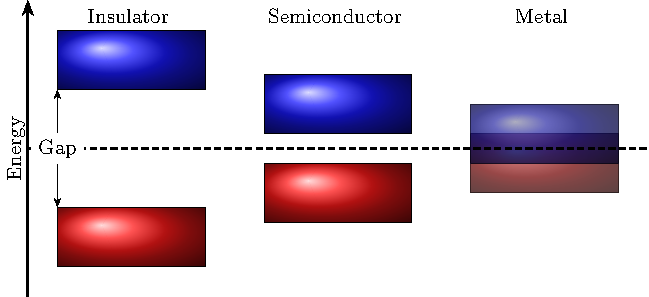
\includegraphics[width=\linewidth]{../figures/chapter-1/solid-sort/build/solid-sort}
	\caption{Band energy diagram for insulators (left), semiconductors(center) and metals (right). The principal difference is the gap energy, for insulators this is longer than semiconductors, although in semiconductors gap energy depends on materials, finally in metals does not exist gap energy instead exist an overlap bands characterize these. Dashed line determines the Fermi level.}
	\label{fig:subsubsection-1.1.1-solid-types}
\end{figure}

The bandgap determines many characteristics and functionalities in semiconductors. In addition, the bandgap energy is classified in direct and indirect, but they do not only depend on this energy but the \gls{BS} is the liable signature for this difference. As pointed out before, it is so difficult to describe electron behavior in solids due to the many body interactions that exists rendering the Scr\"odinger equation very hard to solve. 
Starting by describing bulk semiconductors, for example GaAs, that belongs to the  family III-V cubic semiconductor with a lattice composed by two sublattices with a single atom each (\Cref{fig:subsubsection-1.1.1-bulk-1}). For this case when the atoms in two sublattice are different the crystal structure is called \emph{zinc-blende}\cite{vurgaftman2020bands}.

To calculate \gls{BS} of bulk semiconductors it is important to define specific symmetry directions. For each three-dimensional wave vector $\boldsymbol{k}$, then the plot energy as a function of $\boldsymbol{k}$ is along of different high-symmetry directions\cite{piprek2017handbook}.  GaAs is a direct semiconductor for which the $\left[001\right]$ direction is of high-symetry denoted by $\Gamma$ point ($\boldsymbol{k}=0$)
\begin{figure}[h!]
	\centering
	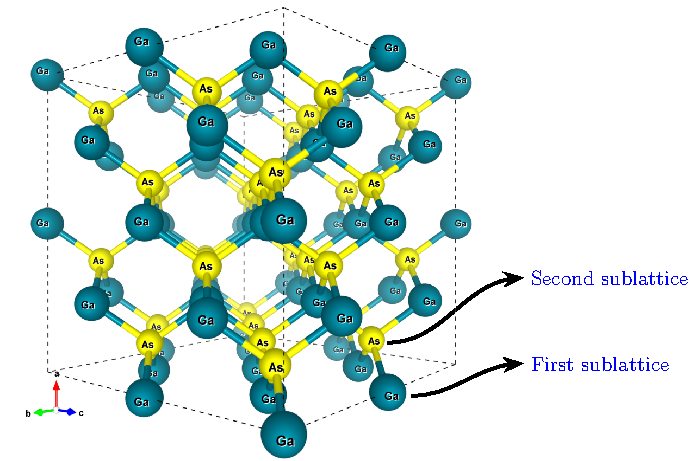
\includegraphics[width=\linewidth]{../figures/chapter-1/bulk-1/build/bulk-1}
	\caption{
		 GaAs crystal structure, where each sublattice corresponds to Ga and As atoms respectively. }
	\label{fig:subsubsection-1.1.1-bulk-1}
\end{figure}

The most ``exact'' computation is carried out by DFT theory. These calculations are  commonly  called atomistic even some  semiempirical models can be regarded as atomistic, but the semiemprical models are also good approximations in comparison with the DFT approach. Then, which is the reason to call ``exact'' solutions to the DFT results? The answer leads us to big discussion, and it is not intended to get into controversy,  but in general the DFT calculations have the capacity to calculate several properties in terms of electrons interaction and the empirical methods are based in the electrical potential choice.\\
 
We will not get into details regarding BS theories and models, but will give a brief reference and the importance to this work. The models much preferred in semiconductor heterostructures such as GaAs/AlGaAs are semiempirical, this is because
\gls{DFT} theory and their derived models are very limited to carry out into large structures, and
their electron interaction nature need high computational performance. Therefore, in comparison
with empirical models where the main role is the potential of semiconductor structures, it reduces computational effort.
%Hence, with empirical models where the main role is the potential of semiconductor structures, this reduces computational effort. 
Then, most models used in semiconductor BS are empirical, and thus these models are distinguished by low computational requirements for this reason are considered as approximated. The importance in discussing these concepts will take relevance when considering physical model proposed in this work. \\*
\begin{figure}[h!]\label{fig:subsubsection-1.1.1-GaAsbands-1}
	\centering
	\begin{subfigure}{\textwidth}
	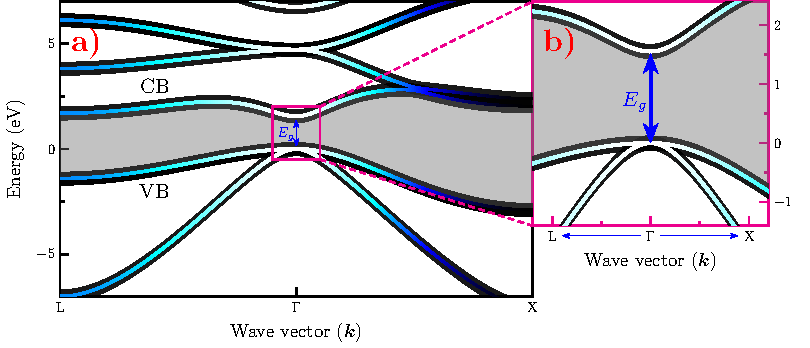
\includegraphics[width=\linewidth]{../figures/chapter-1/bands/build/bands01}
	\phantomsubcaption\label{subfig:subsubsection-1.1.1-GaAsbands-1-a)}
	\phantomsubcaption\label{subfig:subsubsection-1.1.1-GaAsbands-1-b)}
\end{subfigure}
	\caption{Band structure of GaAs, \subref{subfig:subsubsection-1.1.1-GaAsbands-1-a)} shows the zoom around of $\Gamma$  to denote the direct band gap and the electrons energy  needed to jump from valence to conduction band. \subref{subfig:subsubsection-1.1.1-GaAsbands-1-b)} denotes the two directions to dispersion of the bands corresponds to Brillouin zone: $\Gamma\to\mathrm{X}$ and  $\Gamma\to\mathrm{L}$.\cite{fox2002optical}}
\end{figure}
\Cref{fig:subsubsection-1.1.1-GaAsbands-1} shows the results of calculations of \gls{TB} model as discussed in \cite{vogl1983asemiempirical} and the code was implemented by R. Muller \cite{rpmuller2017}. The model proposed by Vogl \textit{et al.},  takes into account a small number of localized pseudo-orbitals  based on the empirical parameters to be  substituted in a TB Hamiltonian.  The importance to calculate the BS is to  predict  reliable and detailed optical properties of solid structures that can be compared with the experimental data.

\Cref{subfig:subsubsection-1.1.1-GaAsbands-1-a)} shows that the GaAs \gls{BS}. \Cref{subfig:subsubsection-1.1.1-GaAsbands-1-b)} depicted, the band dispersion around $\Gamma$ point, which exhibits the highest symmetry.  It is well-known that the band dispersion increasing $\boldsymbol{k}$ along two different directions of the Brillouin zone, from $\boldsymbol{k}=(0,0,0)$ to X point $\boldsymbol{k}=(2\pi a_{L})(1,0,0)$ and L point $\boldsymbol{k}=(2\pi a_{L})(1,1,1)$. These figures are the typical representation of a direct gap III-V semiconductors around  $\boldsymbol{k}=0$ and the shape of the dispersion is parabolic.\\* The BS of GaAs shown in \Cref{fig:subsubsection-1.1.1-GaAsbands-1} does not take into account the contribution of the spin\footnote{This spin contribution as called as split-off (so) hole band.}.  It is important to mention that the characteristic curvature $E\!\!-\!\!\boldsymbol{k}$ of the dispersion bands correspond to an electron ($e$) in case of positive curvature, while the negative curvature corresponds to hole states; heavy (hh) and light hole (lh) bands, denoting that the transitions, are of dipole nature\cite{fox2002optical,cardona2005fundamentals}. 
\begin{figure}[h!]
	\centering
		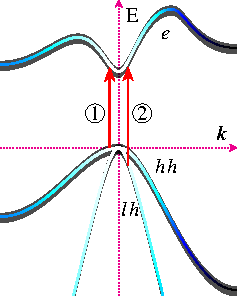
\includegraphics[width=0.5\linewidth]{../figures/chapter-1/bands/build/bands02}
	\caption{Two typical transitions for GaAs near $\boldsymbol{k}=0$. The first one correspond to the heavy-hole and second one to the light-hole. }
	\label{fig:subsubsection-1.1.1-GaAsbands-2}
\end{figure}

All the above discussion refers to a basic quantum mechanism in solids. The electron absorption, specifically interband absorption, offers a way to a fundamental physical process  involving the principle of many basic studies of semiconductors, applications, and the importance to understand the electron behavior in a semiconductor structures disputed in this work. Then \Cref{fig:subsubsection-1.1.1-GaAsbands-2} schematizes the two typical transitions in GaAs bulk, these transitions are near  $k=0$, so that is called interband absorption. It is important to remark that the interband transitions are observed in all solids, but the mechanisms are different depending on their BS, for which,   the BS is the key to study solids  through the very well-know Fermi's golden rule. The excitation of electron in the CB creates a hole VB, then the  final quasiparticle is called \textbf{electron-hole pair}, which is the main subject of the following sections.


\subsection{Excitons}
\label{subsec:chapter-1-excitons}
\vspace{-10mm}
The importance to study \gls{BS} of semiconductors is very clear so far, so that it could be stated that absorption process is the source of optical properties of solids. It is because of this that the importance to study of semiconductors for optoelectronics applications. In addition, this process gives rise to the formation of one of the most important excitations in the crystal structures. The photon absorption process promotes an electron to be excited from  the \gls{CB} to \gls{VB}, generating an empty location in \gls{VB} which has a net positive charge. This positive empty location called as hole, thereby the electron and hole have opposite charge then it is to be expected that they are attracted by Coulomb force, thus creating bound state called an exciton\cite{leonard2017exciton,tanguy1995optical-dispersion}. 

From \Cref{fig:subsubsection-1.1.1-GaAsbands-2} and \Cref{fig:subsubsection-1.1.1-x-1}  it is clear that excitons are commonly present in direct band gap semiconductors such as GaAs, denoted by absorption experiments. This is  mentioned in \Cref{subsec:chapter-3-pl} as the cause in the photoluminescence mechanism.

\begin{figure}[H]
	\centering
	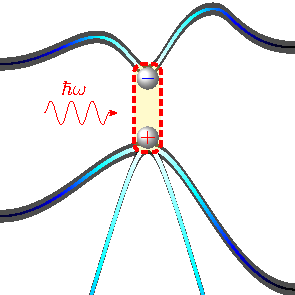
\includegraphics[width=0.5\linewidth]{../figures/chapter-1/exciton-1/build/x-1}
	\caption{Qualitative scheme of exciton creation in GaAs as direct gap.}
	\label{fig:subsubsection-1.1.1-x-1}
\end{figure}

\section{Low Dimensional Semiconductor Structures}
\label{sec:chapter-1-low-dimensional-structures}
\vspace{-10mm} 
The previous section considered the principles of semiconductors; in particular throughout the existence of their \gls{BS}. The first approximations were done for bulk GaAs, for which its symmetry practically defines their nature and consequently the physical effects as excitons existence.  But, what happens  if several semiconductors with the same symmetry and similar structural parameters are joined together?. Do the bulk properties and physical properties are the same?. 
The answers  are well-known: when two materials with relatively same structural parameters, as lattice constant can create a matched heterojunction, the union of several heterojunction make up a heterostructure with a profound impact on the overall optoelectronics properties.\\
\begin{figure}[ht!]
	\centering
	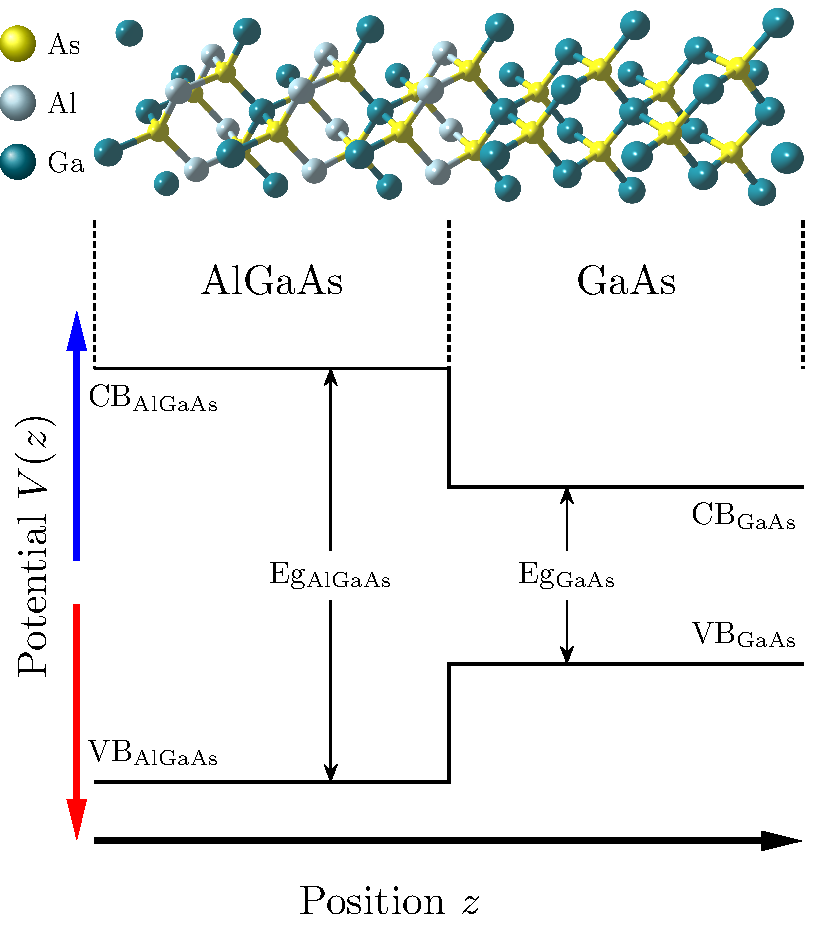
\includegraphics[width=0.6\textwidth]{../figures/chapter-1/heterostructures/build-ruco/hs-01}
	\caption{General scheme of GaAs/\algaas heterostructure. Scheme of atomic arranged of this heterojunction, the dashed lines are the matched between two dissimilar
	materials (top). Band-edge profile (bottom).}
	\label{fig:subsection-1.2-heterostructure}
\end{figure}
\Cref{fig:subsection-1.2-heterostructure} shows  a general scheme for a heterostructure. In this case it is presented three species of atoms Al, As and Ga. These atoms are located in the III-V columns in periodic table, hence they are called III-V semiconductors. The principal characteristic of these atoms is that they can create matched structures such as GaAs, AlAs and ternary alloys as \algaas with specific Al concentration. The matched semiconductors produce a material with new properties based principally in the difference of bandgap which involves the alloys. 
As can see in \Cref{fig:subsection-1.2-heterostructure} it is consisting a GaAs/\algaas heterostructure, these interface is well-matched due to the lattice parameters is relatively equals, therefore and thanks to powerful growth technics as MBE it is possible to get high-quality quantum structures. \\*
Also, the heterostructure composed by two semiconductors with different band gaps generate a discontinuity in either the conduction or the valence band can be represented by a constant potential term\cite{harrison2016quantum}.  The theory for treatment of the electron behavior in these structures is relatively simple if we consider the above. 
Although this chapter has not the intention to explore the theory of electron behavior, it is worth noting that in order to get the one-dimensional potential $V(z)$ for both bands,  the Schr\"odinger equation can be solved accurately. 

\subsection{Quantum Wells}
\label{subsection:chapter-1-quantum-wells}
\vspace{-10mm} 
The major relevance in nanostructured systems lies in the quantum confinement, and 
the junction of semiconductors results in an interesting quantum structures with specific
dimensions. From 3D bulk, the dimensions reduce to 2D, 1D and 0D dimensional structures.
Therefore, each of that has interesting properties and their corresponding applications. 
\Cref{fig:subsection-1.2-heterostructures} shows the low dimensional heterostructures from 3D bulk, the first low dimensional from 3D to 2D is the Quantum Wells, then from 2D to 1D it has the
Quantum Wires finally with 0D have the Quantum Dots. Quantum confinement is the principal reason to study those structures. The electron behavior exhibited in it should help to understand a great variety of quantum mechanical phenomena as electron interaction in a crystal. Suppose a heterostructure composed with a two
semiconductor alloys, this 2D quantum structure is called a Single Quantum
Well (SQW).\\*
\begin{figure}
	\centering
	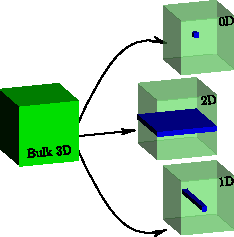
\includegraphics[width=0.6\textwidth]{../figures/chapter-1/heterostructures/build-ruco/lds-00}
	\caption{Heterostructures from bulk (3D), to Quantum Wells (2D), Quantum Wires (1D) and Quantum Dots (0D).  }
	\label{fig:subsection-1.2-heterostructures}
\end{figure}
These  dissimilar semiconductors in terms of their potential energy ($V(z)$) can be schematized in \Cref{fig:subsection-1.2-single-quantum-well-scheme}. The Gap difference of \algaas and GaAs is due to $x$ (Al concentration) in \algaas;  a one dimensional potential profile is obtained, with the possibility to confinement electrons in a 2D plane perpendicular to the  $z$ direction (growth direction). 
If we consider an electron captured by two potential barriers separated a distance $L$, the wavefunction describing such an electron will be spatially confined.
So if we confine many electrons in that potential,  we have two important physical aspects: the first one is knowing as Pauli exclusion principle, which give Fermion nature and prevents carriers with the same spin occupying the same region in  space\cite{harrison2016quantum,pauli1925zusammenhang}. The second  concerns the Heisenberg's uncertainty principle. 
The latter, is the consequence of quantum confinement due to the space reduction of the electrons, which brings that momentum to be increased by an amount of the order $\hbar/L$. Therefore, the energy of that confined particles increases, and it is referred to as confinement energy\cite{cardona2005fundamentals}. \\*
\begin{figure}
	\centering
	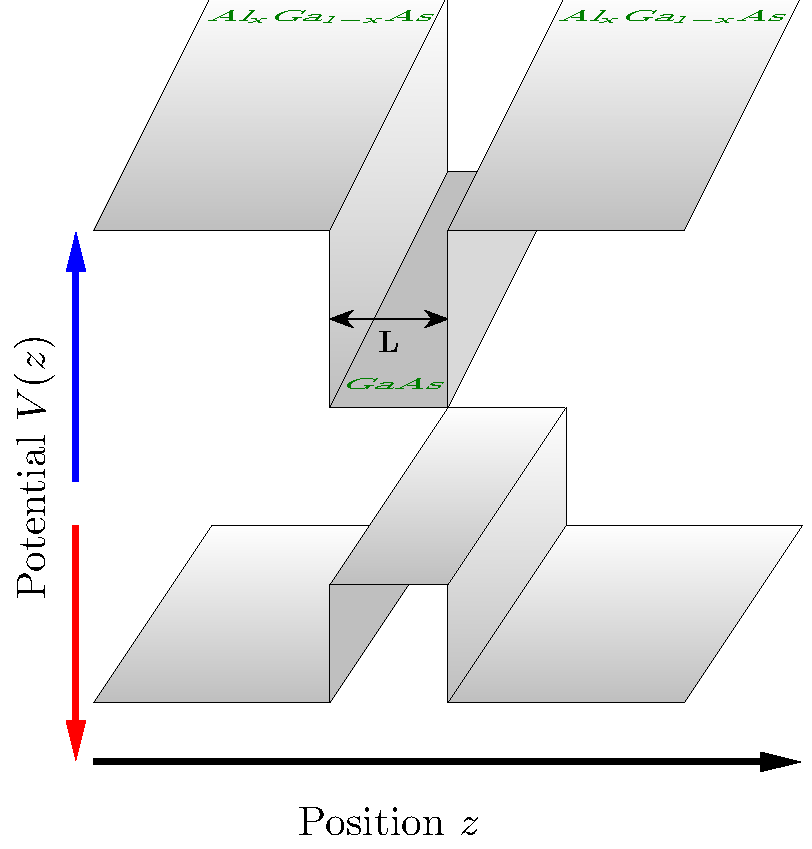
\includegraphics[width=0.65\textwidth]{../figures/chapter-1/heterostructures/out/qw1}
	\caption{Single GaAs/\algaas Quantum Well }
	\label{fig:subsection-1.2-single-quantum-well-scheme}
\end{figure}
Then the quantum confinement is our starting point to understand the optical properties in \gls{QW}s. As is referred in the figure, the uni-dimensional potential profile can well describe by top conduction- and bottom valence-bands, where band offset in these two of correspond gap energy between that, while Al concentration increases their bandgap and the band offset ($\mathrm{Q_{c}}$ to \gls{CB} and $\mathrm{Q_{v}}$ to \gls{VB}) also to.   

It is  now clear  that  \gls{QW}s have the potential to exhibit amazing quantum properties, even if all of these are very important, we focus on the optical properties and basically our interest is the light-matter interaction.  
 
\subsection{Preliminary Approach of Quantum Confinement Effect in QWs}
\label{subsection:chapter-1-preliminary-approach-of-quantum-confinment-effect-in-qws}
\vspace{-10mm} 
We describe the reciprocal space by having two components, $k_{x}$ and $k_{y}$. In the case of GaAs/\algaas \gls{QW}s it is $\Gamma$ point, as long as $x < 0.4$, that the \gls{BS} depends on confinement energy \footnote{It will be explained in the next section, although it is due to the Gap go from direct to indirect, shortly the symmetry $\Gamma\to X$.}.
\begin{figure}[t]
	\begin{subfigure}{\textwidth}
		\centering
		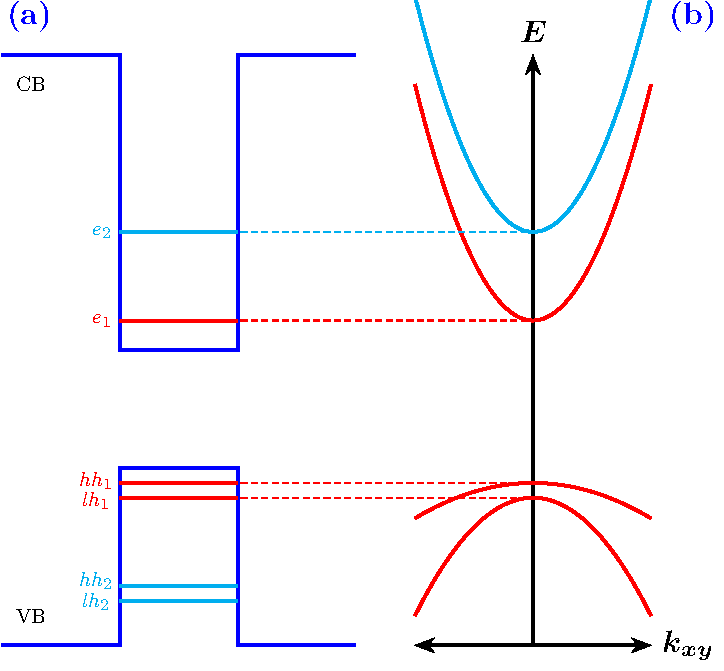
\includegraphics[width=0.65\textwidth]{../figures/chapter-1/heterostructures/out/qw2}
		\phantomsubcaption\label{subfig:subsection-1.2-single-quantum-well-scheme2-a)}
		\phantomsubcaption\label{subfig:subsection-1.2-single-quantum-well-scheme2-b)}
	\end{subfigure}
	\caption{General scheme of typical Schrödinger's equation solutions to one-dimensional potential as \subref{subfig:subsection-1.2-single-quantum-well-scheme2-a)} where the eigenenergies of both electron and holes are denoted with same color depending on  $n$ value.\subref{subfig:subsection-1.2-single-quantum-well-scheme2-b)} it is plot, of the subbands in  the same case of  \subref{subfig:subsection-1.2-single-quantum-well-scheme2-a)} to both particles.  }
	\label{fig:subsection-1.2-single-quantum-well-scheme2}
\end{figure}
In this case, the electronic properties in comparison with a bulk semiconductor properties can be solved trough particle-in-a-box as textbook problem as a first approximation. Nevertheless, even if it can be solved  without  a much mathematical formalism, it is very essential to discuss it here. 
% In general way, as mentioned previously, the Schrödinger equation solution is the fundamental pillar to understand, where it is taken into account which  in a crystal the periodic potential is the key. 
Here we exploit the symmetry properties to understand the corresponding Hamiltonian describing the \gls{QW}.
% Here are important remarks before to continue, when it has a heterostructure starting with the bulk model it is clearly that the system is not the same, the Quantum Mechanics which is behind takes into account the symmetry properties, then it can be developed a Hamiltonian  to understand that system.  In the next chapter will be explained details and the formalism both physical and mathematical to solve and discus it is. 
The model which give the tools to get the solutions is called as Effective Mass Approximation, thus their correspond Schrödinger equation is\cite{harrison2016quantum,chuang1995physics,singh2003electronic,bastard1990wave,fox2002optical,davies1998physics}: 
\begin{equation}\label{eq:chapter-1-ema-schroedinger}
	-\dfrac{\hbar^{2}}{2m^{*}}\dfrac{\partial^{2}}{\partial {z}^{2}}\psi(z)+V(z)\psi(z)=E\psi(z),
\end{equation}

where the $m^{*}$ is the effective mass in each material, and $V(z)$ is the potential profile deduced from  heterostructure materials properties. Therefore, that differential equation can be solved as in textbooks \cite{de2014introduccion,griffiths2018introduction,sakurai1995modern,cohen2019quantum,chuang1995physics,harrison2016quantum,fox2002optical,bastard1990wave}. The idea is to think as a one particle in a finite potential well with definite and established  boundary conditions and solving the Schrödinger equation in each part of single \gls{QW}, this means that we need to create a potential function. Thus the Eigenfunctions and their corresponding Eigenenergies are computed.

The principal idea is not reproducing something which is very well known, the objective of this part is to established the scope of the next chapter. Therefore,  before to continue, we will finish explaining the dispersion in-plane of single \gls{QW}. As in the \gls{QW} the one-dimensional potential set up the 1D confinement, is important do not confuse which the \gls{QW} is a 2D structure, but their confinement is along of $z$ direction, this means a 1D. Then, the particle can motion in the $x-y$ plane. By this reason, even if consider 3D Schrödinger equation and  the above is considered it obtain \Cref{eq:chapter-1-ema-schroedinger}
therefore, the solutions in the one-dimensional potential produce discrete states of energy $E_{z}=E_{n}$\cite{harrison2016quantum}, where $n$ is the energy level it which produce  subbands as shows in \Cref{fig:subsection-1.2-single-quantum-well-scheme2}. In contrast, before it called as ``energy bands'' in the bulk case, now due to the quantum confinement gets subbands to both conduction- and valence bands.

These subbands are the result of the sum of $E_{z}$ and $E_{x,y}$, which are the 1D confinement energy and the in-plane momentum $k_{x,y}$ then\cite{harrison2016quantum}:
\begin{equation}\label{eqn:chapter-1-total-enery-ema-aprox}		
	E = E_{n} + \dfrac{\hbar^{2}|\boldsymbol{k}_{x,y}|^{2}}{2m^{*}}.
\end{equation}  
From this equation the effective mass  $m^*$ depends on particle, i.e the effective mass to electrons in CB and the holes in VB. Hence, the most relevant parameter in the solution is the energy $E_{n}$ (\Cref{subfig:subsection-1.2-single-quantum-well-scheme2-b)}) which discrete, thus yielding the quantum confinement in the low-dimensional
heterostructures.
\section{Summary}
\vspace{-10mm} 
This chapter exposed the generalities of semiconductor band structure and low-dimensional
heterostructures, highlighting GaAs/\algaas, which is of importance in this work. The band structure interpretation
is usually hard to tackle  but the impact and relevance in optical properties of semiconductors starts from that interpretation, Another significant concept which was treated as first approach, is the effective mass concept, even if solved, the bulk
Hamiltonian it considers the mass as constant parameter or depending on semiconductor
material, contrary in low-dimensional structures have an important role.

In general, the band structure of semiconductors is key to understand quantum
properties of solids, and for this work the relevant issued  is the \emph{light-matter} interaction within the linear regime. Remember that \emph{light-matter} interaction in solids can be studied by process resulting in it, as absorption,
reflection, transmission, diffraction, scattering, and others \cite{rivera2020light}. Although, the light-matter
interactions are fundamentally quantum electrodynamical, also, it can be studied in quantum
way through aforementioned process. Firstly, is the photon absorption process can help
to understand or calculate the fundamental parameter in semiconductors as is bandgap
energy. This parameter is the started point in the study of semiconductors, this is the start
point in the map called \gls{BS}, if it ignores the gap value in the semiconductor to
study it couldn't possibly get the principal optical properties of that.
% Then, the \gls{BS} of semiconductors is the map to understand them, without these
% routes or fundamental parameter, we could not have quantum devices at hand.
Then, the \gls{BS} of semiconductors is the map to understand them and without these routes to assess fundamental
parameters, we could not have quantum devices at hand.